\documentclass{article}
\usepackage{lscape}
\usepackage[utf8]{inputenc}
\usepackage{tikz}
\usetikzlibrary{shapes.geometric}
\usepackage{pgfplots}
\usepackage{graphicx}
\graphicspath{ {images/} }
\usepackage{imakeidx}
\usepackage{comment}
\usepackage{amsmath}
\usepackage{framed}
\usepackage{subcaption} 
\usepackage[style=authoryear,sorting=nyt]{biblatex}
\addbibresource{ref.bib}


\title{Institutions and Growth: a GMM/IV Panel VAR Approach}
\author{Carlos Góes\footnote{International Monetary Fund (WHD). I thank Maddie Eldridge \parencite*{maddie} for giving me the initial insight that one should try to incorporate the feedback loops between institutions and growth to this debate, which pointed to a VAR-type analysis. I am grateful to Troy Matheson, Alfredo Cuevas, Ranae Jabri, Alex Herman, Aart Kraay, Leo Feler, and the anonymous referee for their helpful comments. All potential mistakes and omissions are solely mine.}}
\date{Economics Letters R\&R Version: November 2015}

\begin{document}

\maketitle

\begin{abstract}
Both sides of the institutions and growth debate have resorted largely to microeconometric techniques in testing hypotheses. In this paper, I build a panel structural vector autoregression (SVAR) model for a short panel of 119 countries over 10 years and find support for the institutions hypothesis. Controlling for individual fixed effects, I find that exogenous shocks to a proxy for institutional quality have a positive and statistically significant effect on GDP per capita. On average, a 1\% shock in institutional quality leads to a peak 1.7\% increase in GDP per capita after six years. Results are robust to using a different proxy for institutional quality. There are different dynamics for advanced economies and developing countries. This suggests diminishing returns to institutional quality improvements. \\
Keywords: Institutions, Panel VAR, Economic Development. \\
JEL Codes: O43, C33, C14.
\end{abstract}

\newpage

\section{Introduction}

Since Acemoglu, Johnson and Robinson's \parencite*{acemoglu} seminal paper supporting the link between institutions and development, the debate over the role in institutions on economic growth has spurred much research. Those who are critic of institutionalism are perhaps better represented by Jeffrey Sachs \parencite*{sachs} and some of his co-authors, who have emphasized the prevalence of ecology and geography over institutions in economic development. Others, like Nunn and Puga \parencite*{np}, have taken a more nuanced position on this split, by arguing that geography has historically played a key role in shaping institutions and thus can indirectly explain income differences between countries.

In spite of the very prolific work on this field, most of the literature has resorted solely to microeconometric techniques in testing hypotheses. There are several reasons for that. The most important one is that complete time series of country-wide institutional quality indicators have only become available in the last fifteen years. This has limited the extent to which researchers can explore dynamics in the institutions-growth relationship since the data are still too scant for individual-country time-series analysis. Additionally, although the popularity of  panel vector autoregressions has been increasing since the seminal work of Holtz-Eakin \textit{et al} \parencite*{he}\footnote{See Canova and Ciccarelli \parencite*{canova} for a comprehensive literature review.}, its use is still remarkably rarer than traditional VARs.

Like Chong and Calderón \parencite*{cc}, who show evidence of bi-directional Granger causality between institutions and growth, I take a macroeconometric approach to this debate. I extend their insight by building a Panel Structural Vector Autoregression (SVAR) model for 119 countries over 10 years using Arellano-Bond's dynamic panel equations. The largest contribution of this approach is showing that institutions and growth have a \textit{dynamic and bi-directional} relationship and providing reliable estimates of it. While most of the literature focuses on how institutions help explain differences \textit{between countries} over the very long run, results here presented show how and to which extent, on average, changes in institutions over time help explain changes in income \textit{within} the same country.

The advantages of this approach are manifold. By using Arellano-Bond, it estimates unbiased fixed-effects average coefficients for dynamic panels. The results control for all the  time-invariant characteristics that are usually considered in the development literature. They include, for instance: latitude, access to sea, temperature, humidity, ruggedness, language, culture of colonizing power, etc. This approach permits the calculation of unbiased impulse response functions (IRFs), which take full advantage of the information contained in the cross-sectional dimension of the sample. Finally, as with any VAR, it assumes endogeneity of the all variables in the system and allows for studying the dynamics of purely exogenous shocks.

Using the Economic Freedom of the World Index as a proxy for institutions, I find that exogenous shocks to institutional quality have a positive and statistically significant effect on GDP per capita. On average, a 1\% shock in institutional quality, as measured by this proxy index, leads to a peak 1.7\% increase in GDP per capita after six years. Such peak response is robust to using a different proxy for institutions (the Corruption Perception Index). There are, however, different dynamics for advanced and developing countries, with the peak statistically significant responses being 0.4\% and 2.6\%, respectively, suggesting diminishing returns to institutional quality improvements. 

\section{Methodology}

I estimate the following model:

\begin{eqnarray}
    B y_{i,t} &=& f_i + A(L)  y_{i,t-1} + e_{i,t}, \\
    i &=& [1, ... , 119]', t = [2002, ... , 2012]' \nonumber
\end{eqnarray}

where $y_{i,t} \equiv [c_{i,t} , k_{i,t}]'$ is a bi-dimensional vector of stacked endogenous variables, $c_{i,t}$ is the log of GDP per capita in constant 2005 U.S. dollars, $k_{i,t}$ is the proxy for institutional quality, $f_i$ is a diagonal matrix of time-invariant individual-specific intercepts, $A(L) = (\sum_{j=0}^p A_{j} L^j)$ is a polynomial of lagged coefficients, $A_{j}$ is a matrix of coefficients, and $e_{i,t}$ is a vector of stacked residuals, and $B$ is a matrix of contemporaneous coefficients.

However, since $f_i$ is correlated to the error terms, estimation through OLS leads to biased coefficients. As explained in Baltagi \parencite*{baltagi}, first-differencing and using lagged instruments is a good strategy to get consistent parameters and eliminate individual fixed-effects when $N$ is large and $T$ is fixed. Following that line, I estimate a system of $m = 2$ equations with Arellano-Bond's GMM/IV technique\footnote{As described in Arellano and Bond \parencite*{ab}, the GMM estimators assume $E[e_{m,i,t}|Z] = 0$, where $Z$ is a matrix of instruments which are correlated with regressors and orthogonal to the error terms. For each equation, the moment estimators will minimize the above assumption by changing the symmetric matrix $M$ in $[(X'ZMZ'X')^{-1}X'ZMZ'Y']$, where $X$ is a matrix of all lagged variables on the right hand-side and $Y$ is a vector of the variable on the left-hand side. Bond \parencite*{bond} shows that GMM estimators for autoregressive models, including Arellano-Bond, extend in a natural way to include "a vector of current and lagged values of additional explanatory variables". Even if regressors are endogenous and correlated with the contemporaneous residuals, lagged regressors are efficient instruments that can be included in $Z$.}.  Each equation in the system has the first difference of an endogenous variable on the left hand side, $p$ lagged first differences of all $m$ endogenous variables on the right hand side, and no constant.

\begin{eqnarray}
    \Delta y_{1,i,t} &=& \sum_{j=1}^p \gamma^j_{11} \Delta y_{1,i,t-j} + \hdots + \sum_{j=1}^p \gamma^j_{1m} \Delta y_{m,i,t-j} + e_{1,i,t}, \nonumber \\ 
    &\vdots& \\
\Delta y_{m,i,t} &=& \sum_{j=1}^p \gamma^j_{m1} \Delta y_{1,i,t-j} + \hdots + \sum_{j=1}^p \gamma^j_{mm} \Delta y_{m,i,t-j} + e_{m,i,t}, \nonumber
\end{eqnarray}

In its equivalent vector moving average (VMA) representation, the Panel SVAR model can be rendered as follows:

\begin{eqnarray}
    By_{i,t} &=& \Phi (L) e_{i,{t}} 
\end{eqnarray}

where $\Phi(L) = \sum_{j=0}^{\infty} \Phi_{j} L^j = \sum_{j=0}^{\infty} A_{1}^j L^j$ is a polynomial of reduced-form responses to stochastic innovations and $\Phi_0 = A_1^0 \equiv I_m$.

To recover the $B$ matrix and identify the model, I first retrieve the variance-covariance matrix $\Sigma_e = E[e_{i,t}e_{i,t}']$. Since  $B^{-1}e_{i,t} = u_{i,t}$, then $\Sigma_e = E[Bu_{i,t}u_{i,t}'{B}']$. As the structural residuals $u$ are assumed to be uncorrelated ($u_{i,t}u_{i,t}' = I_m$), I derive the $B$ matrix by decomposing the variance-covariance matrix into two triangular matrices.

To identify the model I need to impose one restriction to orthogonalize the contemporaneous responses. In the Cholesky ordering, institutional quality is set to have no contemporaneous effect on GDP per capita while the latter is allowed to contemporaneously impact the former. By construction, this \textbf{reduces} the short-term impact of institutional quality on GDP per capita, so this design is more robust if one is trying to test the institutional hypothesis. However, in the absence of strong \textit{a priori} reasons why institutions should not affect income contemporaneously, I present the results using the alternative ordering of variables in the robustness section.

In recovering the impulse responses from the matrices, I follow the method explained by Lutkepöhl \parencite*{lutkepohl}. Take the following rendering of the VMA representation of the Panel SVAR:  

\begin{eqnarray}
    B M(L) y_{i,t} &=& e_{i,t} \\
    B y_{i,t} &=& M(L)^{-1} e_{i,t} \nonumber 
\end{eqnarray}

where $M(L) \equiv (I_m - \sum_{j=1}^\infty A_{j} L^j)$. Since $B y_{i,t} = \Phi(L) e_{i,{t}}$, it follows that $M(L)^{-1} = \Phi(L)$ and $M(L)^{-1}\Phi(L) = I_m$. After factorizing the identity and truncating the impulse horizon to $h$ periods, I can recover matrices of marginal responses $\Phi_h$ recursively:

\begin{eqnarray}
    \Phi_h &=&  \sum_{i=1}^h \Phi_{h-i}A_h
\end{eqnarray}

I then multiply all $\Phi_j$ by $B^{-1}$ and use a bi-dimensional impulse vector $s \equiv [1, 0]'$ to construct a matrix $P$ of structural responses:

\begin{equation}
    P = 
    \begin{bmatrix}
        B^{-1} \Phi_0 s \\
        B^{-1} \Phi_1 s \\
            \vdots \\
        B^{-1} \Phi_h s \\
    \end{bmatrix}_{hxm}
\end{equation}

Collecting the first column into a vector ($\rho^1 \equiv [\rho_{11}, ... , \rho_{h1}]'$), I have the IRF of the first endogenous variable to a shock in the first endogenous variable. Afterwards, I repeat the process until the $m^{th}$ variable ($\rho^m \equiv [\rho_{1m}, ... , \rho_{hm}]'$). I then change the impulse variable by replacing vector $s$ above. After recovering the point estimates of all the impulse response functions, I calculate standard errors through a resampling simulation with 1000 repetitions.

\section{Data}

I use GDP per capita data in constant 2005 U.S. dollars from the World Bank's World Development Indicators as the income variable and the Fraser Institute's Economic Freedom of the World Index (EFW) as a proxy for institutional quality. The index takes into account five institutions-related subcomponents, namely: legal system reliability, monetary stability, burden of regulation, size of government, and freedom to trade internationally\footnote{See Gwartney, Lawson, and Hall \parencite*{efw} for details.}.

I chose EFW for two reasons. First, it is significantly correlated with the risk of appropriation index AJR used in their original paper ($t-stat > 7$). It is also correlated to other potential proxies for institutions, such as the Economist Intelligence Unit's Democracy Index or Transparency International's Corruption Perception Index (CPI), which was used in the robustness section. In fact, the first principal component of those four indices explain about 70\% of the total variance, suggesting that those different metrics are measuring similar underlying characteristics. If the index AJR used in their paper or any of the other indices mentioned are a good proxies for institutions, so should be the EFW index.

Second, it provides a continuous annual time series between 2000 and 2012 for a very wide range of countries. Since the Arellano-Bond estimators perform better on short panels (i.e., panels with large $N$ and small $T$), I wanted to take advantage of the information available from the variability between individuals as much as possible. The large cross sectional dimension of the EFW index fits suit.  

The data are organized into a panel of 119 countries and 12 years. The Arellano-Bond framework implies a necessity to transform the data into first differences and use lagged instruments. For such reason, the final estimation sample drops to 10 years, resulting a total of 1190 observations. 

\newpage

\begin{figure}[ht]
\begin{center}
    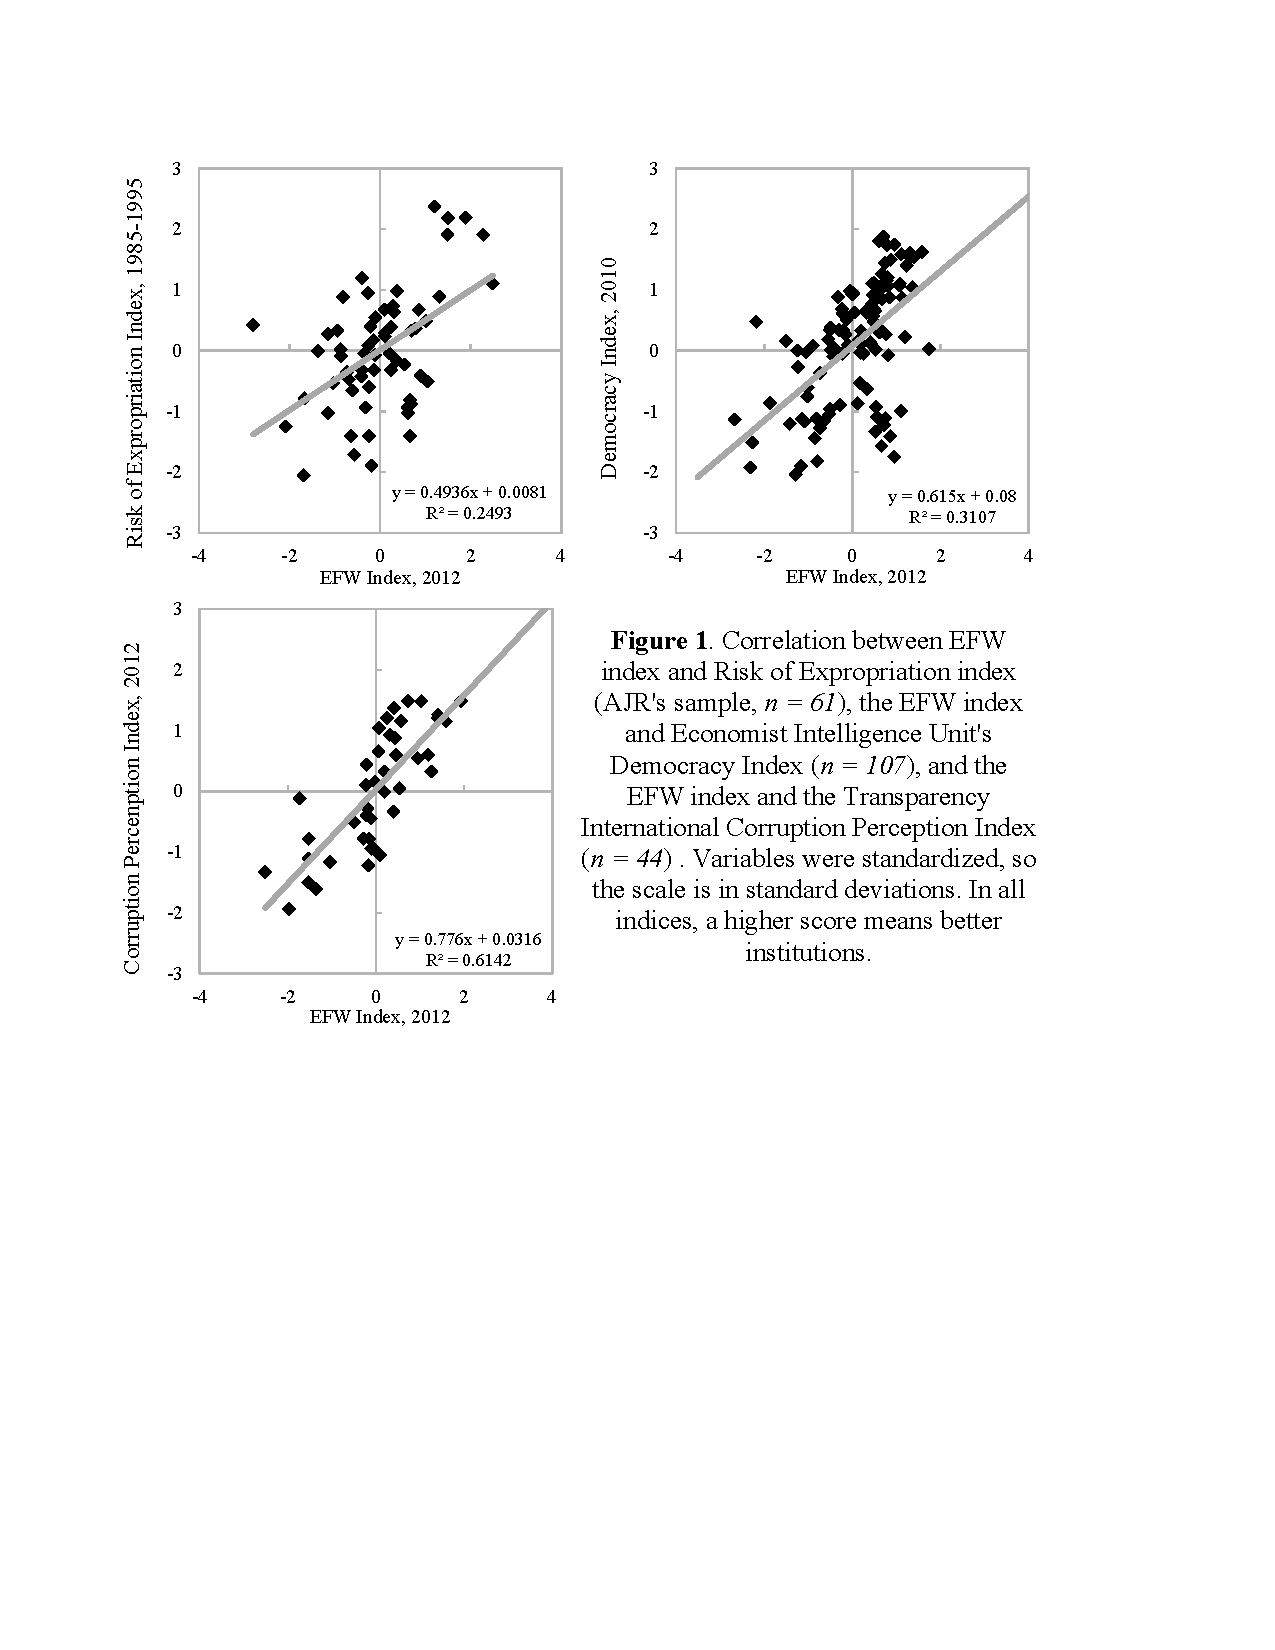
\includegraphics[scale=0.7]{correlation.pdf}
%    \caption{Correlation between EFW index and Risk of Expropriation index (AJR's sample, $n = 61$) and between EFW index and Economist Intelligence Unit's Democracy Index ($n = 107$) . Variables were standardized, so the scale is in standard deviations. In all indices, a higher score means better institutions.}
\end{center}
\end{figure}


\section{Results}

The results from the estimated GMM/IV Panel VAR are \textit{average responses} of endogenous variables to an \textit{exogenous shock} in any variable \textit{after controlling for time-invariant characteristics of individual members}. It takes into consideration all the simultaneous dynamics in the system. J-statistics of the GMM regressions suggest the instrumentation strategy is valid. Since the Panel SVAR is stable, shocks eventually converge to zero. This means that shocks are temporary and over the long run the series return to their deterministic trends.

It is not obvious what a shock in institutional quality is. Such shock is an innovation in institutional quality as captured by the proxy of choice. The results in this section suggest improvements in institutions can lead to higher income per capita, which is also observed in the contemporaneous correlation between the two variables, as seen in Figure 2 below. The standard deviation in changes in the institutions proxy is 3.5\% and the average annual improvement is 0.4\%. 

\begin{figure}[ht]
\begin{center}
    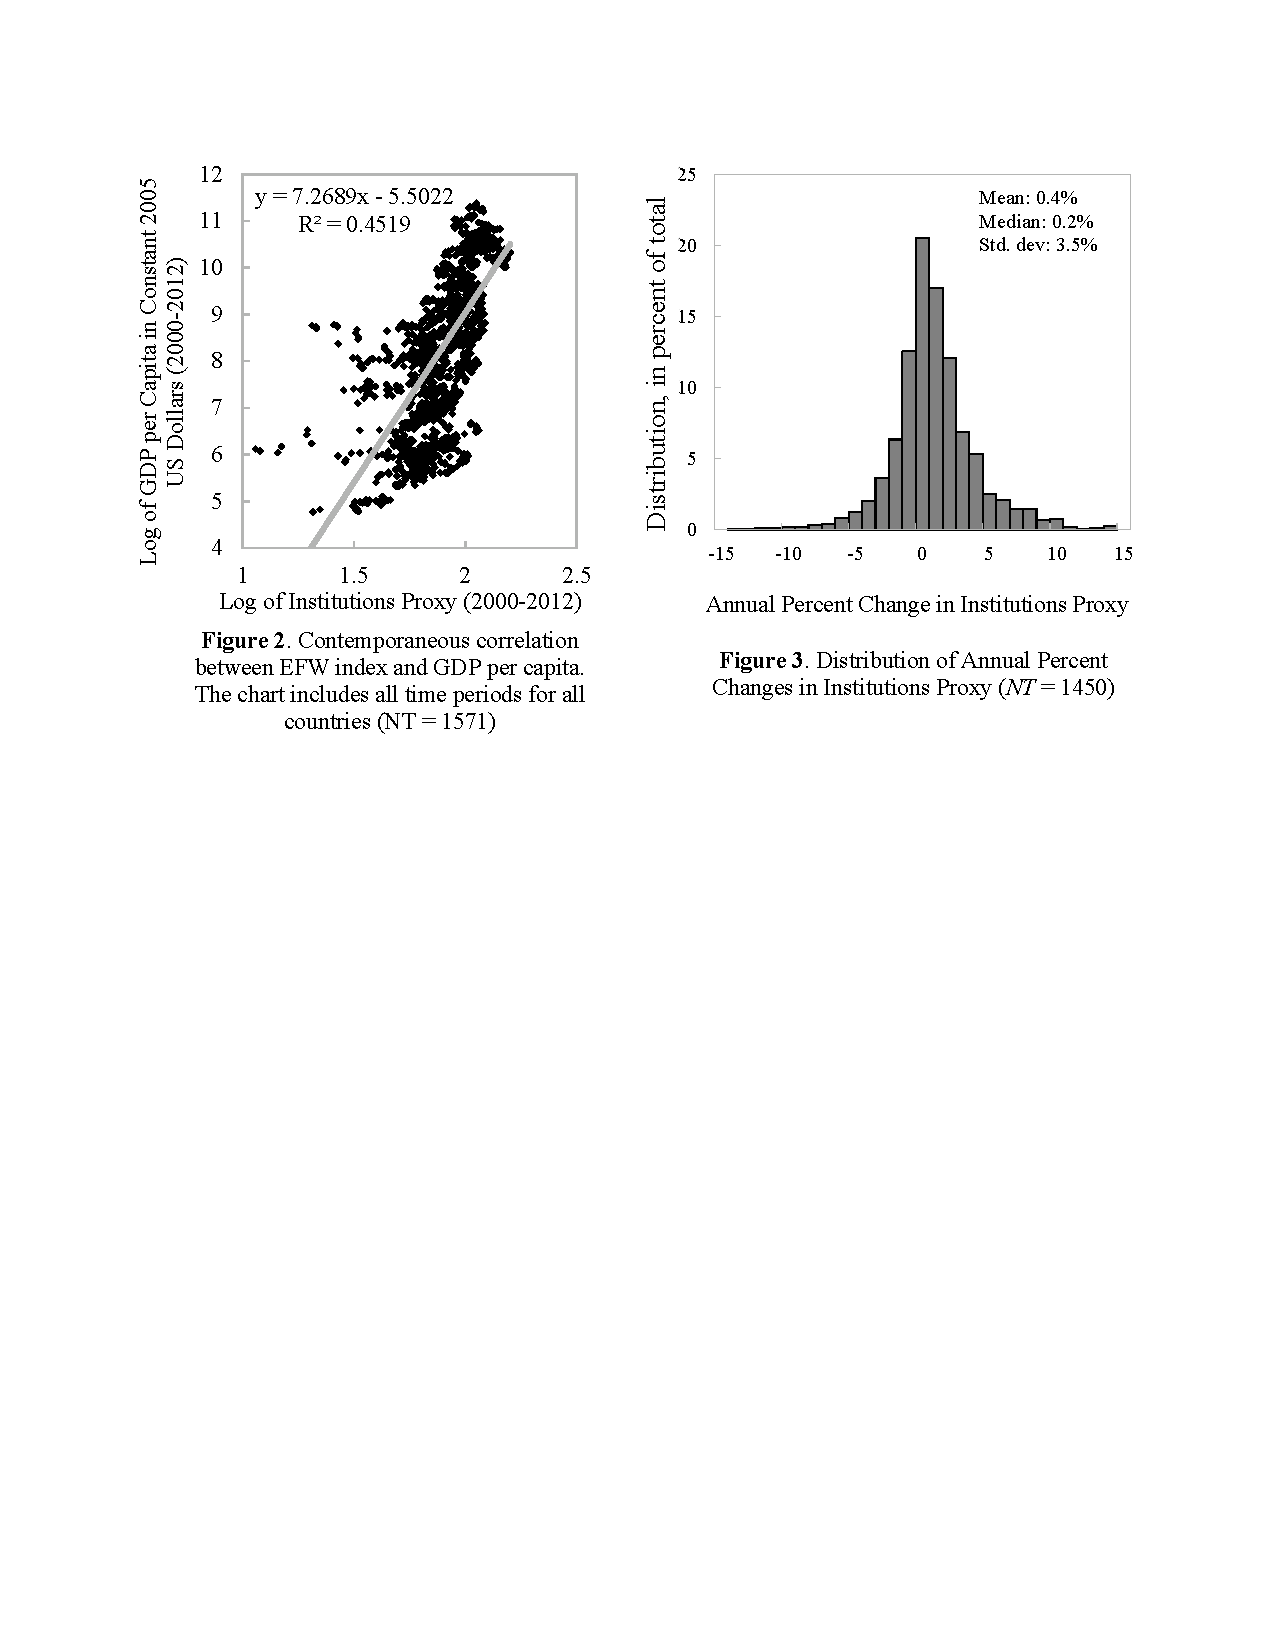
\includegraphics[scale=0.675]{distribution.pdf}
\end{center}
\end{figure}

Taking the EFW index as a proxy, the institutional gap between Nicaragua and Costa Rica, for instance, is about 10\%. Similarly, Burundi is about 30\% below Rwanda. At the average pace of institutional improvement of 0.4\% per year, it would take about 25 years for a 10\% gap to close, if all other countries remained unchanged. This is intuitive, since institutions are generally expected to move slowly.

I find that, on average, a 1\% shock in institutional quality leads to a peak 1.7\% increase in GDP per capita after six years. The relationship remains positive and statistically significant up until 10 years after the shock, though decreasingly so. After the $4^{th}$ year uncertainty increases rapidly, as shown by the broadening confidence bands. By contrast, GDP per capita affects institutional quality almost entirely through the contemporaneous relationship, with following years being driven primarily by the latter's own autoregressive process.

\newpage

\begin{figure}[!hb]
\begin{center}
    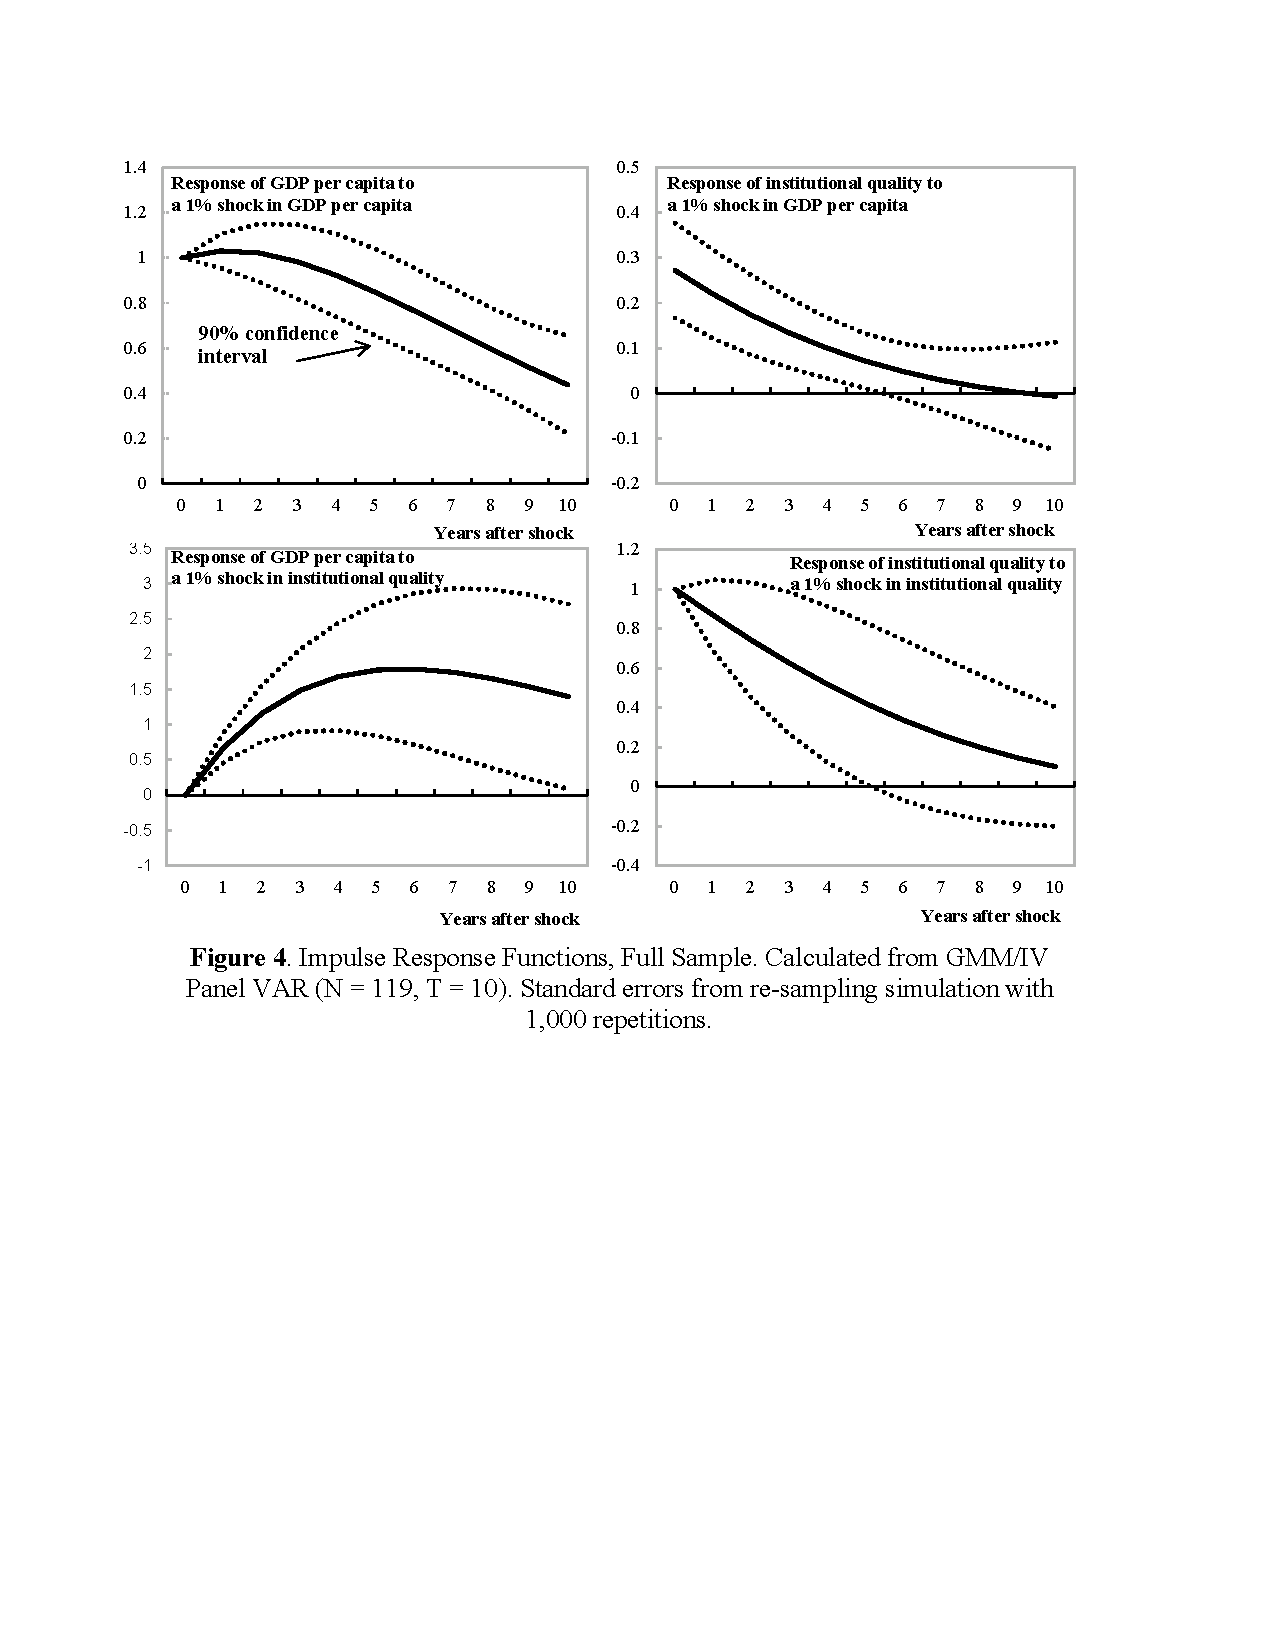
\includegraphics[scale=0.675]{whole.pdf}
\end{center}
\end{figure}

One of the setbacks of the GMM/IV approach is that it imposes homogeneous dynamics across individuals. To address this shortcoming, I split the sample between advanced and developing countries. I find that, as expected, the dynamics are indeed different among different country groups.

When restricting the sample to 25 advanced economies, the impact of improved institutional quality in GDP per capita is much smaller than observed in the whole sample, peaking at 0.35\% two years following a 1\% shock. Interestingly, after shocks both on GDP per capita and on institutional quality, institutional quality quickly returns back to its trend. Results are in Figure 5 below.

\newpage

\begin{figure}[ht!]
\begin{center}
    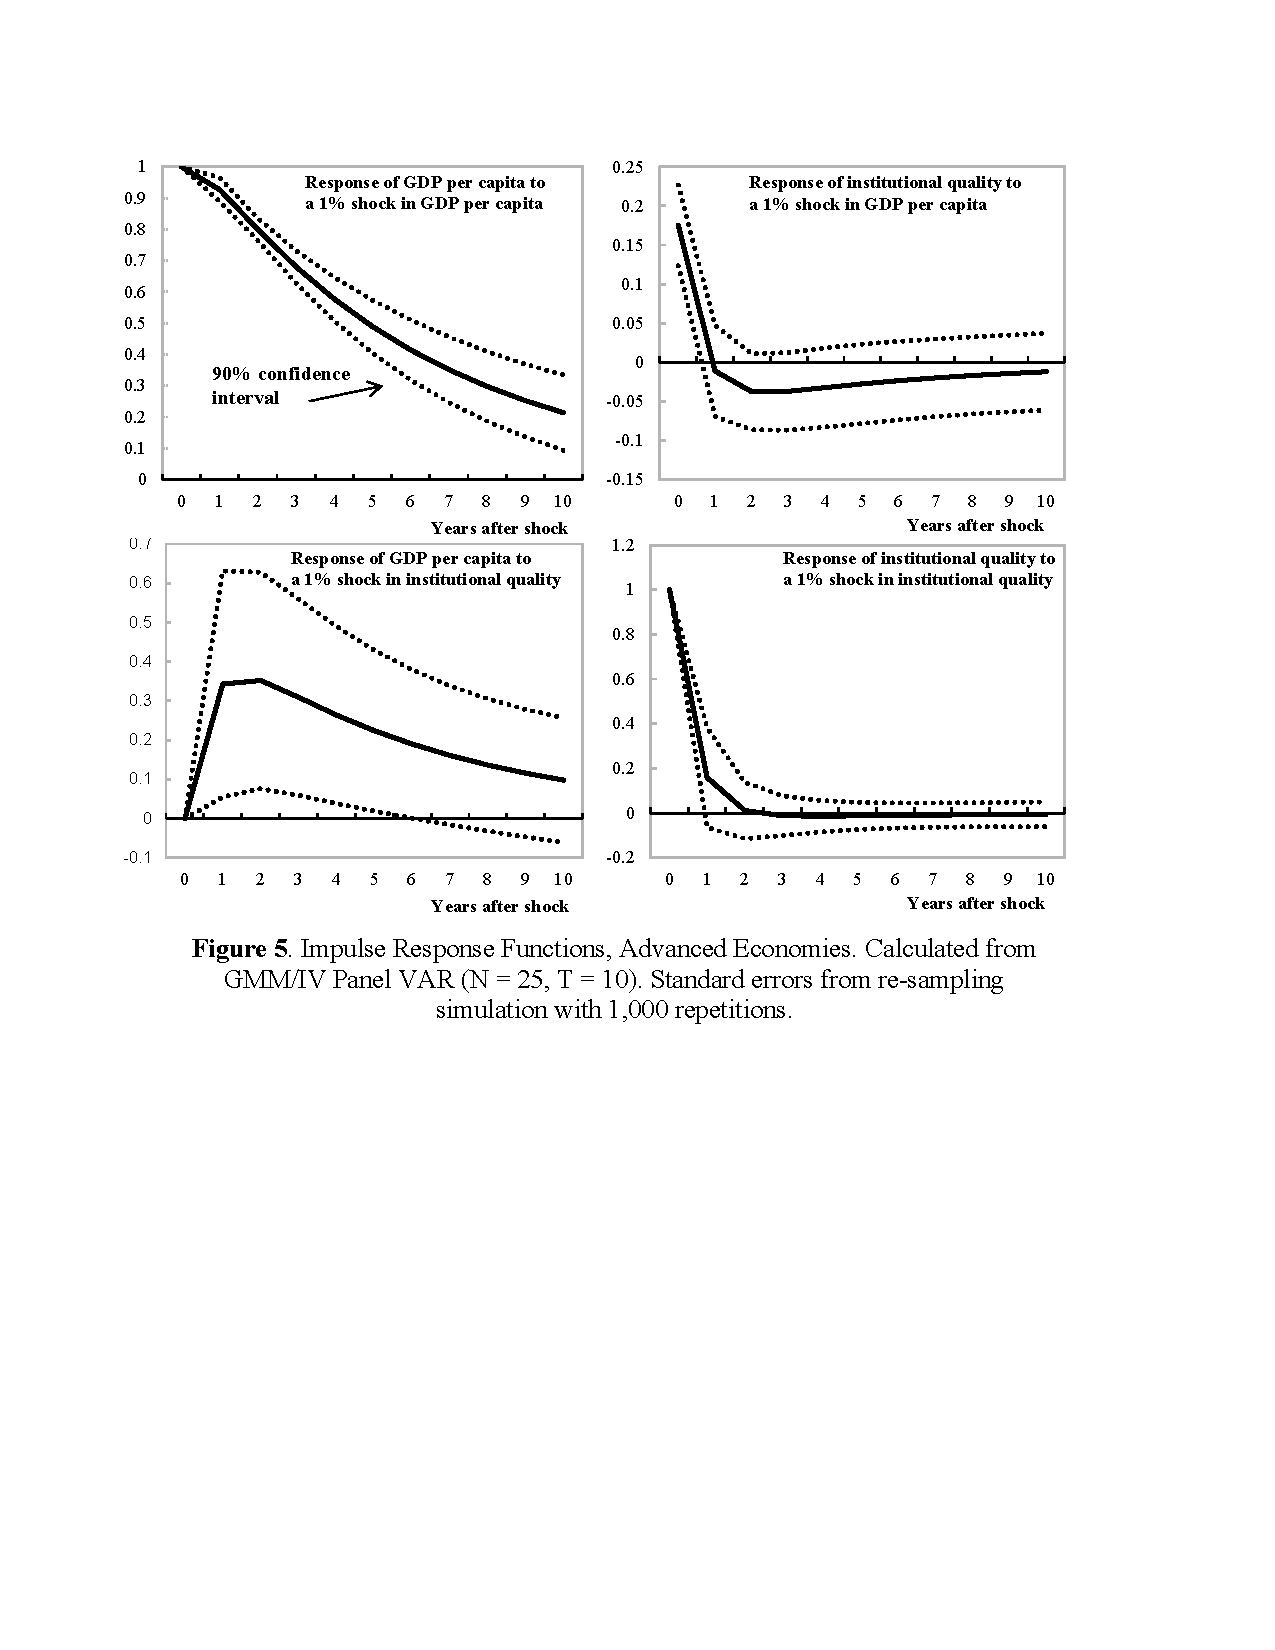
\includegraphics[scale=0.675]{advanced.pdf}
\end{center}
\end{figure}

This is strikingly different from the results of estimating the model with the remaining 94 developing countries. For developing countries, the peak statistically significant response is 2.6\%. Standard errors are much larger throughout all responses, which is expected, since developing countries tend to be more heterogeneous than advanced economies. 

\newpage


\begin{figure}[ht]
\begin{center}
    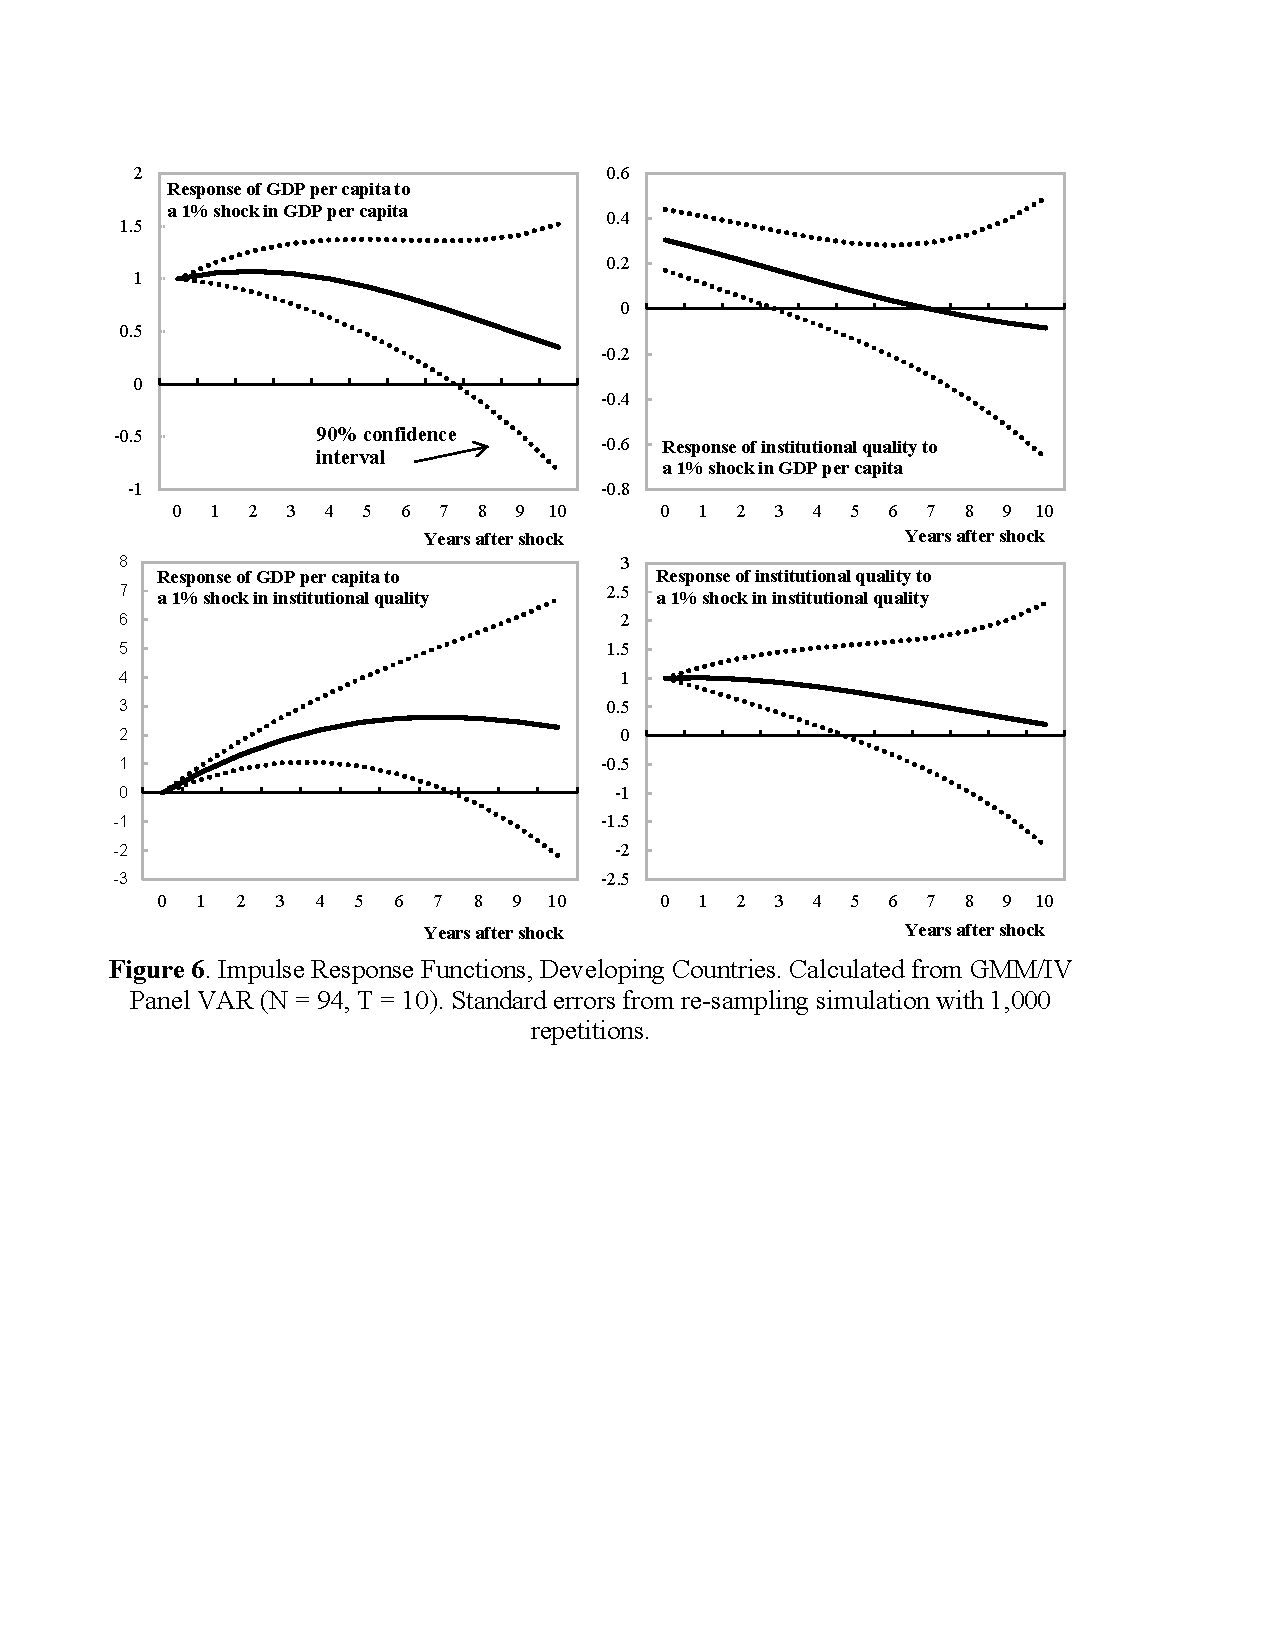
\includegraphics[scale=0.675]{developing.pdf}
\end{center}
\end{figure}

\section{Robustness}

I test the robustness of the results with two alternative specifications. First, I invert the Cholesky ordering of endogenous variables. The baseline specification restricts  contemporaneous effects of institutions on income, while the alternative specification does the inverse. Since those variables are contemporaneously correlated, restrictions will tend to limit the positive impact of a variable on the other. As expected, the alternative specification shows a higher peak response of income to institutional quality (1.9\% vs. 1.7\% in the baseline) and a lower peak response of institutional quality to income (0.2\% vs. 0.3\% in the baseline). Such small differences do not change the overall interpretation of results.

Afterwards, I assess robustness by replacing the proxy for institutions used in the baseline model. The model design and specification is the same. I replace EFW with the Transparency International's Corruption Perception Index (CPI), which is a composite index that tries to assess how fair, trustworthy and transparent governments in different countries are. When using the CPI as the proxy the response of income to innovations in institutions is also positive and statistically significant. 

The peak response of GDP per capita to a 1\% shock in institutional quality leads is 1.3\%, slightly \textit{smaller} than the baseline model. Conversely, peak response of institutional quality to a 1\% shock in GDP per capita is 0.35\%, slightly \textit{larger} than the baseline. They both fall well within the 90\% confidence interval of the baseline model. All results are in the charts below.

\begin{figure}[ht]
\begin{center}
    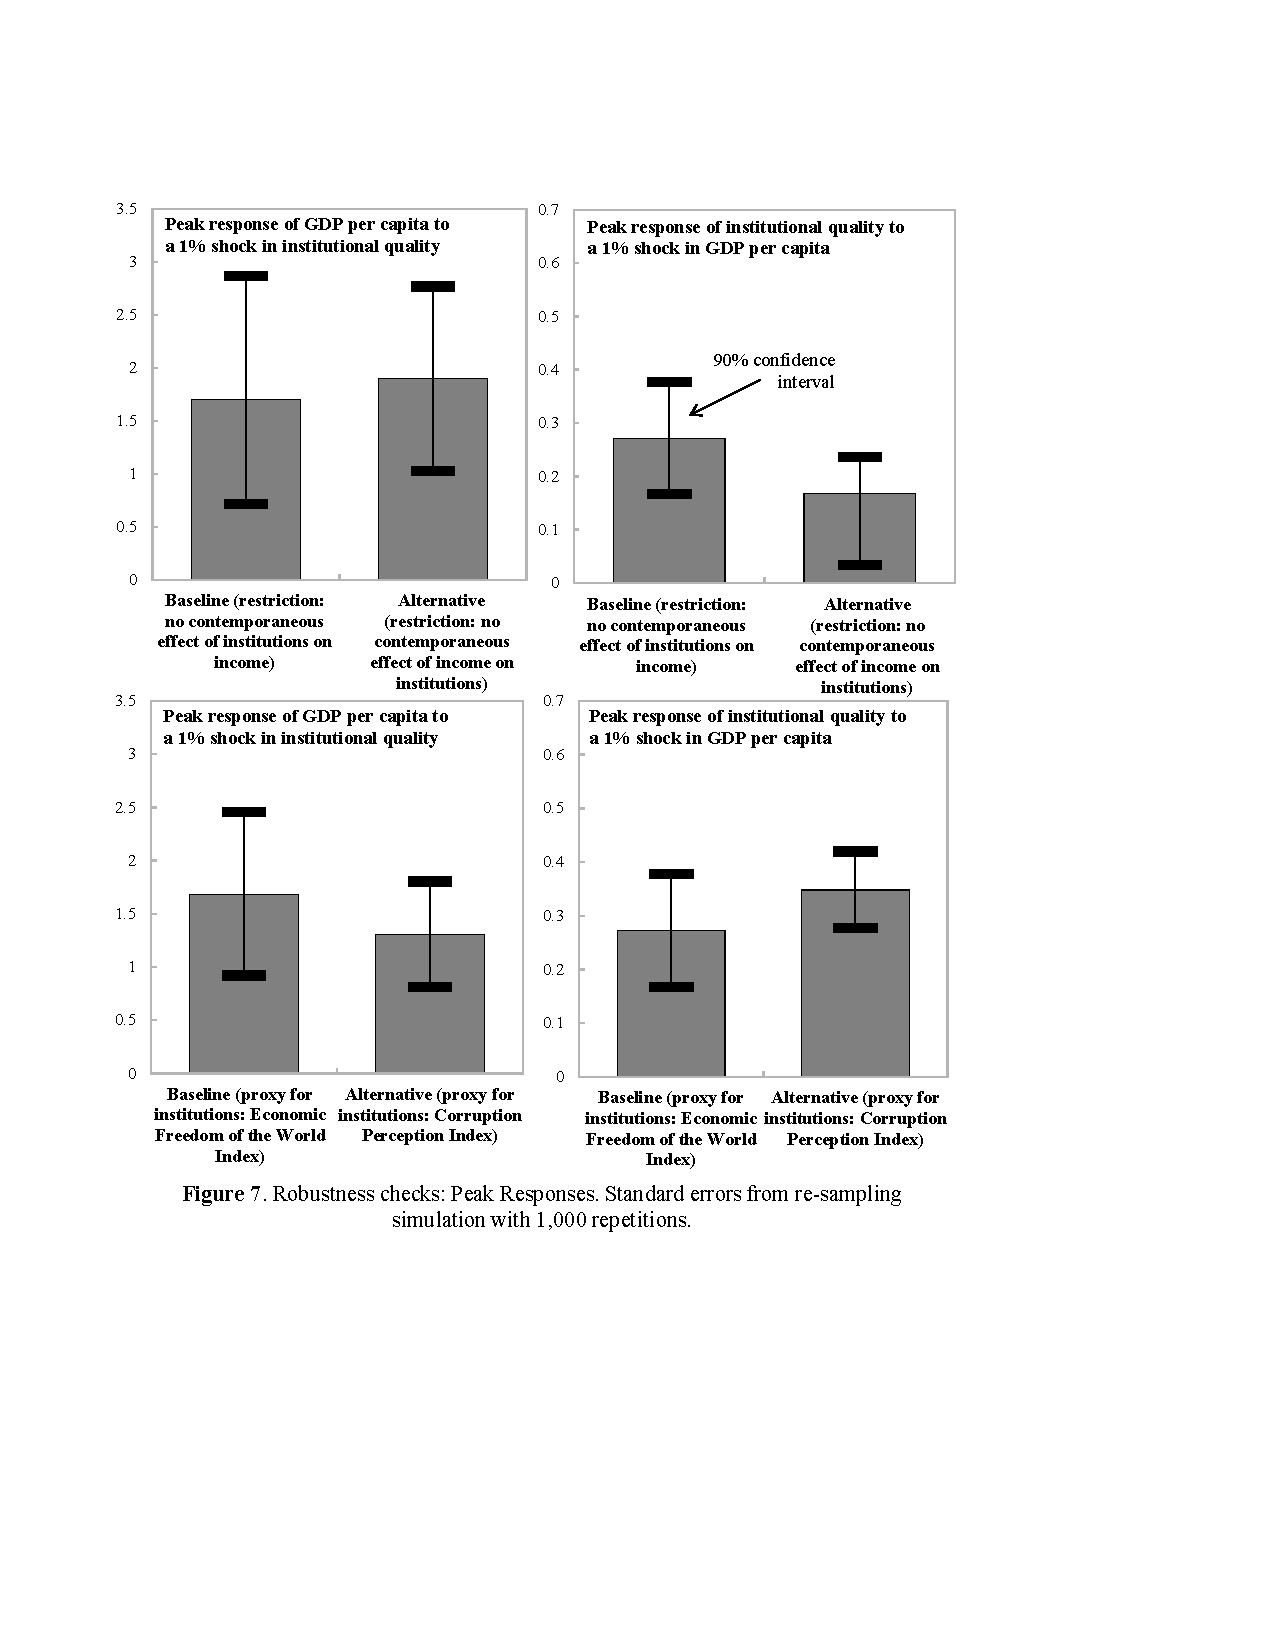
\includegraphics[scale=0.8]{robustness.pdf}
\end{center}
\end{figure}

Measuring institutional quality can be problematic, but the consistency in the direction of responses using different proxies and orderings suggest that, qualitatively, the relationship between institutions and growth are similar. Such qualitative result is more important than the magnitude of the responses themselves.

\section{Conclusion}

I find evidence that exogenous improvements in institutional quality have positive and statistically significant impact on GDP per capita. The model controls for all time-invariant individual characteristics which are usually taken as controls in the economic development literature, does not suffer with endogeneity problem, and is robust to using a different proxy for institutions. Moreover, different proxies tend to be significantly correlated, which suggests results would not be qualitatively different when replacing proxies. 

This novel approach supports the institutions hypothesis in dynamically determining development and provides evidence for bi-directional causality between institutions and growth. Additionally, the heterogeneous responses between advanced and developed economies suggest diminishing returns to institutional quality improvements, which is consistent with standard income convergence intuition. Countries with higher GDP per capita tend to have higher institutional quality, but for those countries the payoff in terms of (percentage) increase in GDP per capita is smaller. By symmetry, developing countries have higher payoffs when improving institutional quality.

\printbibliography

\newpage

\appendix
\numberwithin{equation}{section}
\section{Appendix: Standard error simulation algorithm}

I use a resampling Monte Carlo algorithm with the following steps:

\begin{enumerate}
    \item I draw a random $k$-dimensional vector $r \equiv [r_1 , ... , r_k]'$, where $r \in \mathbb{Z}$ and all $r_k$ follow a discrete uniform distribution $U\{1,N\}$, where $N = 119$ is the number of cross-sections in the sample. I set $k$ to $10\%$ of the sample size plus one cross-section ($k = .1N + 1$) and truncate the result by discarding any decimal points.
    \item I exclude $k$ cross-sections from our original sample, thus restricting  the sample to $T(i-k)$ observations.
    \item I re-estimate the model with the restricted sample, collect the matrices of responses, extract individual vectors for each IRF and organize the simulated IRFs into a separate matrix for each $m$ endogenous variable.
    \item After I repeat this procedure $n = 1000$ times the result will be $2$ distribution matrices $D$: 

\begin{equation}
    D_m = 
    \begin{bmatrix}
        \tilde{\rho}^1_{1m} & \hdots & \tilde{\rho}^n_{1m} \\
        \vdots & \ddots & \vdots \\
        \tilde{\rho}^1_{hm} & \hdots & \tilde{\rho}^n_{hm} 
    \end{bmatrix}_{hxn}
\end{equation}

where $m$ is the $m^{th}$ response variable, $h$ is the response horizon, and $n$ is the number of repetitions of the simulation exercise.

\item From $D_m$ I take square root of the second moment of each row to build a vector of standard errors: 

\begin{equation}
    \sigma_{\rho_{m}} = 
    \begin{bmatrix}
        \text{Var}[\{\tilde{\rho}^1_{1m} , \hdots, \tilde{\rho}^n_{1m}\}]^{1/2} \\
        \vdots\\
        \text{Var}[\{\tilde{\rho}^1_{hm}, \hdots, \tilde{\rho}^n_{hm}\}]^{1/2} 
    \end{bmatrix}_{hx1}
\end{equation}
\end{enumerate}

\end{document}


%%%%%%%%%%%%%%%%%%%%%%%%%%%%%%%%%%%%%%%%%%%%%%%%%%%%%%%%

